
%============================================================
\subsection{\texttt{cube}}
\label{subsec:geometry_cube}
%============================================================

\noindent
\textbf{Geometry ID:} \texttt{GLOB-GEO0002}
\qquad
\textbf{Version:} \texttt{1.0.0}

\begin{figure}[htbp]
    \centering
    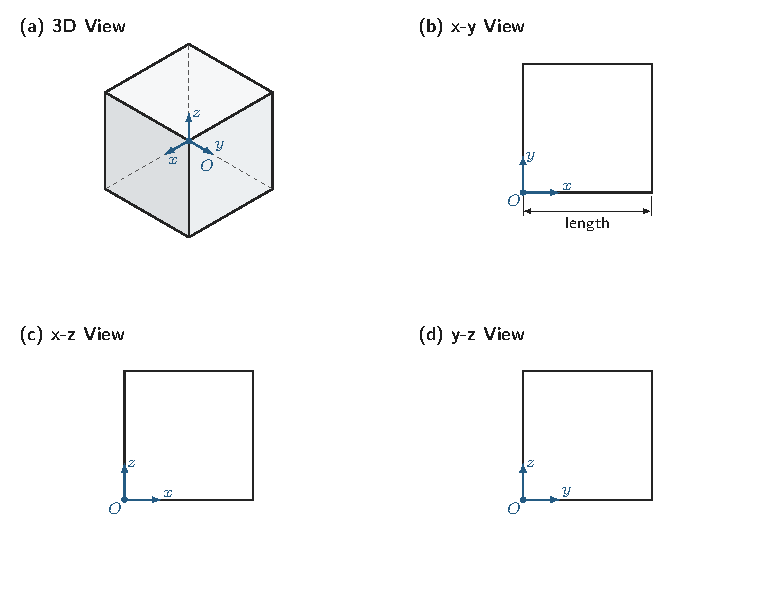
\includegraphics[width=0.7\linewidth]
    {./figs/geometries/cube.pdf}
    \caption{Standardized parametrization and local
    coordinate system of the cube geometry.}
    \label{fig:cube}
\end{figure}

The \texttt{cube} geometry represents a cubic
specimen with equal dimensions along three mutually
orthogonal directions. As illustrated in
Fig.~\ref{fig:cube}, the local coordinate system
is defined by the right-handed Cartesian axes
$x$, $y$, and $z$, with the origin located at
the reference corner indicated in the figure.

The three coordinate axes are aligned with the
edges of the cube.

\paragraph{Independent parameters.}

The geometry is defined by one required parameter,
expressed in millimeters:

\begin{itemize}
    \item \texttt{length}: cube edge length,
    corresponding to the dimensions along
    the local $x$, $y$, and $z$ directions.
\end{itemize}

\paragraph{Geometric constraints.}

The parameter \texttt{length} must be strictly
positive.
